% ŠABLONA PRO PSANÍ ZÁVĚREČNÉ STUDIJNÍ PRÁCE
%%%%%%%%%%%%%%%%%%%%%%%%%%%%%%%%%%%%%%%%%%%%
% Autor: Jakub Dokulil (kubadokulil99@gmail.com)
% Tato šablona byla vytvořena tak, aby pomocí ní mohli v systému LaTeX soutěžící sázet své práce a zároveň odpovídala požadavkům na formátování vyplývajícím z wordové šablony umístěné na webu soc.cz.
%
\documentclass[12pt, a4paper, twoside]{report}

%% Proměnné
\newcommand{\code}[1]{\colorbox{lightgray}{\texttt{#1}}}
\newcommand\obor{INFORMAČNÍ TECHNOLOGIE} %% -- napiš číslo a název tvého oboru
\newcommand\kodOboru{18-20-M/01} %% -- napiš číslo a název tvého oboru
\newcommand\zamereni{se zaměřením na počítačové sítě a programování} %% -- napiš číslo a název tvého oboru
\newcommand\skola{Střední škola průmyslová a umělecká, Opava} %% vyplň název školy
\newcommand\trida{IT4} %% vyplň jméno svého konzultanta
\newcommand\jmenoAutora{Jiří Ryba}  %% vyplň své jméno
\newcommand\skolniRok{2023/24} %% vyplň rok
\newcommand\datumOdevzdani{1. 1. 2024} %% vyplň rok
\newcommand\nazevPrace{modelGate} %% vyplň název své práce
\newcommand\podnazevPrace{posuvná brána s elektrickým pohonem}

\title{\nazevPrace} %% -- Název tvé práce
\author{\jmenoAutora} %% -- tvé jméno
\date{\datumOdevzdani} %% -- rok, kdy píšeš SOČku

%% Balíčky
\usepackage[top=2.5cm, bottom=2.5cm, left=3cm, right=3cm]{geometry} %% nastaví okraje, left -- vnitřní okraj, right -- vnější okraj

\usepackage[czech]{babel} %% balík babel pro sazbu v češtině
\usepackage[utf8]{inputenc} %% balíky pro kódování textu
\usepackage[T1]{fontenc}
\usepackage{cmap} %% balíček zajišťující, že vytvořené PDF bude prohledávatelné a kopírovatelné

\usepackage{graphicx} %% balík pro vkládání obrázků

\usepackage{subcaption} %% balíček pro vkládání podobrázků

\usepackage{hyperref} %% balíček, který v PDF vytváří odkazy

\linespread{1} %% řádkování
\setlength{\parskip}{0.5em} %% odsazení mezi odstavci


\usepackage[pagestyles]{titlesec} %% balíček pro úpravu stylu kapitol a sekcí
\titleformat{\chapter}[block]{\scshape\bfseries\LARGE}{\thechapter}{10pt}{\vspace{0pt}}
\titleformat{\section}[block]{\scshape\bfseries\Large}{\thesection}{10pt}{\vspace{0pt}}
\titleformat{\subsection}[block]{\bfseries\large}{\thesubsection}{10pt}{\vspace{0pt}}

\usepackage{tocloft} % Balíček umožní přizpůsobit vzhled tabulky obsahu
\setlength{\cftbeforechapskip}{0pt}  % Menší rozestup pro kapitoly
\setlength{\cftbeforesecskip}{0pt}   % Menší rozestup pro sekce

\setcounter{secnumdepth}{2}
\setcounter{tocdepth}{2}
\usepackage{fancyhdr}
\pagestyle{fancy}
\renewcommand{\headrulewidth}{0.025pt}

\usepackage{booktabs}

\usepackage{url}

%% Balíčky co se můžou hodit :) 
%%%%%%%%%%%%%%%%%%%%%%%%%%%%%%%

\usepackage{helvet} % Helvet font
\usepackage{mathptmx} % Times New Roman
\usepackage{Oswald} % Oswald font

\usepackage{listings}
\usepackage{xcolor}

\renewcommand{\lstlistingname}{Kód}% Listing -> Algorithm
\renewcommand{\lstlistlistingname}{Seznam programových kódů}% List of Listings -> List of Algorithms

%% Definice 
\lstdefinestyle{c++}{
	language=C++,                % C++ code
	commentstyle=\color{red}, % style for comments
	keywordstyle=\color{blue},   % style for keywords
	numberstyle=\tiny\color{red}% style for line numbers
	basicstyle=\tiny\ttfamily
}

%% Začátek dokumentu
%%%%%%%%%%%%%%%%%%%%
\begin{document}
	
	\lstset{basicstyle=\small}
	
	\pagestyle{empty}
	\pagenumbering{Roman}
	
		
	%% Titulní stránka s informacemi
	%%%%%%%%%%%%%%%%%%%%%%%%%%%%%%%%%%%%%%%%
	
	{\fontfamily{phv}\selectfont
		%% Logo školy
		\begin{figure}[h]
			\centering
			
\includegraphics[width=0.6\linewidth]{image/logo-skoly.png} 
		\end{figure}
		
		%% Hlavička práce a její název (viz proměnná \nazev prace)
		%% \sffamily %%% bezpatkové písmo - sans serif
		{\bfseries %%% písmo na stránce je tučně
			\begin{center}
				\vspace{0.025 \textheight}
				\LARGE{ZÁVĚREČNÁ STUDIJNÍ PRÁCE}\\
				\large{dokumentace}\\
				\vspace{0.075 \textheight}
				\LARGE {\nazevPrace}\\
				\large{\podnazevPrace}\\
			\end{center}  
		}%%%
		
		\vspace{0.05 \textheight}
		
		\begin{figure}[h]
			\centering
			
\includegraphics[width=0.6\linewidth]{image/modelGateLogo.png} 
		\end{figure}
		
		\vspace{0.2 \textheight}
		\begin{table}[h!]
			\centering
			\begin{tabular}{ll}
				\textbf{Autor:} & \jmenoAutora\\ 
				\textbf{Obor:} & \kodOboru { } \obor\\
				\textbf{} & \zamereni\\
				\textbf{Třída:} & \trida\\
				\textbf{Školní rok:} & \skolniRok\\
			\end{tabular}
			
		\end{table}	
	}
	
	
	
	%% Stránka obsahující poděkování a prohlášení
	%%%%%%%%%%%%%%%%%%%%%%%%%%%%%%%%%%%%%%%%%%%%%%%%%%%%%%%%
	
	\newpage
	
	%% Poděkování - nepovinné
	%%%%%%%%%%%%%%%%%%%%%%%%%%%%
	
	\noindent{\Large{\bfseries{Poděkování}\\}}
	\noindent Rád bych poděkoval učitelům Mgr. Marcelu Godovskému a Mgr. Marku Lučnému za jejich pomoc s projektem, jelikož mi poskytovali součástky a cenné rady.\\
	
	\vspace{0.6 \textheight}
	
	%% Prohlášení - povinné
	%%%%%%%%%%%%%%%%%%%%%%%%%%%%
	\noindent{\large{\bfseries{Prohlášení}\\}}
	\noindent Prohlašuji, že jsem závěrečnou práci vypracoval samostatně a uvedl veškeré použité informační zdroje.\\
	\noindent Souhlasím, aby tato studijní práce byla použita k výukovým a prezentačním účelům na Střední průmyslové a umělecké škole v Opavě, Praskova 399/8.
	\vfill
	\noindent{V Opavě \datumOdevzdani\\}
	\noindent
	\begin{minipage}{\linewidth}
		\hspace{9.5cm} 
		\begin{tabular}{@{}p{6cm}@{}}
			\dotfill \\
			Podpis autora
		\end{tabular}
	\end{minipage}
	
	%% Stránka obsahující anotaci
	%%%%%%%%%%%%%%%%%%%%%%%%%%%%%%%%%%%%%%%%%%%%%%%%%%%%%%%%	
	
	\newpage
	
	%% Anotace
	%%%%%%%%%%%%%%%%%%%%%%%%%%%%
	\noindent{\Large{\bfseries{Abstrakt}\\}}
	\noindent Projekt se zaměřuje na kompletní realizaci posuvné brány s elektrickým pohonem, zahrnující návrh, modelování, sestavení a programování. Je zde využit mikrokontrolér Arduino Nano, který umožňuje integraci s dálkovým ovládáním, koncovými spínači a senzorem pohybu. Výsledkem projektu je plně funkční 3D model posuvné brány, schopný reagovat na vstupy a poskytující efektivní automatizaci otevírání a zavírání.  \\
	
	\noindent{\large{\bfseries{Klíčová slova}}}
	
	\noindent Arduino Nano, modelování, programování, sestavení \dots 
	
	\vspace{0.04 \textheight}
	\noindent{\Large{\bfseries{Abstract}\\}}
	\noindent The project focuses on the complete implementation of an electrically operated sliding gate, including design, modelling, assembly and programming. An Arduino Nano microcontroller is used, which allows integration with remote control, limit switches and motion sensor. The project results in a fully functional 3D model of a sliding gate, capable of responding to inputs and providing efficient automation of opening and closing. \\
	
	\vspace{18pt}
	
	\noindent{\large{\bfseries{Key words}}}
	
	\noindent Arduino Nano, modelling, programming, assembling \dots 
	
	%% Vlastní obsah
	%%%%%%%%%%%%%%%%%%%%%%%%%%%%%%%%%%%%%%%
	
	%% Poděkování DONE
	%% Prohlášení DONE
	%% Anotace DONE
	%% Úvod DONE
	%%   Přehled Projektu - popsání co tam je a co to umí DONE 
	%%   Účel - k čemu projekt slouží (proč jsem to začal dělat atd. inspirace) DONE
	%% Tvorba modelu DONE
	%%   3D Modelování DONE
	%%		Výběr softwaru DONE 
	%%		Výhody a nevýhody autodesk inventoru DONE 
	%%		Modelování konstrukce DONE
	%%		Modelování brány DONE
	%%		Modelování ozubeného kolečka a ozubené lišty DONE
	%%		Modelování destiček a čepiček DONE
	%%   3D Tisk DONE
	%%   Sestavení DONE %% přidat fotku
	%% Harwdare DONE
	%%   Seznam použitého hardwaru DONE
	%%   Schéma DONE
	%%   Arduino Nano DONE
	%%   Problémy spojené s hardwarem DONE
	%%		Ovladač neovladačuje DONE
	%% 		Napájení motoru %% arduino má malý proud (Ampery) DONE
	%% Funkce Modelu Brány DONE
	%%   Otevření, zavření a zastavení DONE
	%%   Bezpečností Senzor na Pohyb DONE
	%%   LED Indikátory a Motor DONE
	%%   Poskládání kódu DONE
	%%   Shrnutí DONE
	%% Možné vylepšení (apka na telefon, otevírání na spzky) (Závěr) DONE
	%% Zdroje a citace
	
	%% SEZNAM HARDWARE
	%% 1x Arduino Nano (mikrokontrolér)
	%% 2x DM00 (spínače)
	%% 1x L298N (h můstek)
	%% 1x 5V motor %%najít přesně
	%% 3x LED %%najít přesně
	%% 3x 330R Rezistor
	%% 3X 1k Rezistor
	%% 1x HW-201 (senzor na pohyb)
	%% 1x VS1838B (IR příjimač)
	%% 1x Vytisknutá konstrukce
	%% 1x Vytisknutá brána
	%% 1x Vytiskunté ozubené kolečko
	%% 1x Vytisknutá ozubená tyč
	%% 4x Vytisknuté plotové destičky
	%% 3x Vytisknuté čepičky na plot
	
	%% Stránka s generovaným obsahem
	%%%%%%%%%%%%%%%%%%%%%%%%%%%%%%%%%%%%%%%
	
	\newpage
	
	\let\oldchapter\chapter		
	\renewcommand{\chapter}{
		\pagestyle{plain}
		\oldchapter
	}
	
	\tableofcontents %% Vygeneruje tabulku s obsahem
	
	\thispagestyle{empty}
	
	%% Stránka s úvodem
	%%%%%%%%%%%%%%%%%%%%%%%%%%%%%%%%%%%%%%%		
	
	\newpage
	
	\pagenumbering{arabic} %% Nastavení způsobu číslování stránek (alternativy roman | Roman)
	\setcounter{page}{5} %% Nastavení počitadla stránek
	
	\chapter*{Úvod}
	\addcontentsline{toc}{chapter}{Úvod}
	
	\noindent Cílem tohoto projektu bylo proměnit myšlenku v realitu. Jednoho dne, když jsem řešil stavbu skutečné posuvné brány na rodinném pozemku, mě napadlo, že bych podobný koncept mohl zkusit vytvořit jako menší projekt. Po schválení nápadu od všech učitelů jsem se do toho pustil.\\
	
	\noindent Pro samotné provedení modelu jsem vytvořil 3D modely, které mi vytiskl pan učitel Mgr.~Marcel Godovský na 3D tiskárně. Vytisknuté modely poskytly fyzickou podobu brány a umožnily snadné sestavení. Programování mikrokontroléru Arduino Nano~bylo klíčovým krokem k dosažení ovládání brány. Vytvořil jsem řídící algoritmus, který umožňuje plynulé otevírání a zavírání brány v reakci na externí podněty, například signály~ze snímačů nebo dálkového ovladače. \\
	
	\noindent Dokumentace obsahuje použité komponenty, zapojení a způsob programování mikrokontroléru. Kromě toho jsou zahrnuty i možné vylepšení projektu. Tato dokumentace slouží jako průvodce pro každého, kdo má zájem o pochopení a reprodukci podobného projektu posuvné brány s využitím Arduino technologie. \\

	%% Stránka Tvorba modelu
	%%%%%%%%%%%%%%%%%%%%%%%%%%%%%%%%%%%%%%%
	
	\chapter{Tvorba modelu}
	
	\section{3D modelování}
	
	\subsection{Výběr softwaru}
	
	\noindent Při výběru modelovacího softwaru pro můj projekt jsem měl na výběr mezi několika možnostmi, mezi nimiž byly klíčovými kandidáty 3DS Max, Blender a Autodesk Inventor. Po~důkladném zvážení všech faktorů jsem se rozhodl pro Autodesk Inventor. \\
	
	\subsection{Výhody a nevýhody Autodesk Inventoru}
	
	\noindent Rozhodl jsem se využít Autodesk Inventor, díky mé předchozí zkušenosti s tímto programem. Tato volba mi umožnila efektivní modelování bez nutnosti učení se nového softwaru. Díky studentské licenci poskytnuté školou jsem nemusel platit za software. Autodesk Inventor, specializovaný na inženýrství a konstrukci, odpovídá potřebám mého projektu s parametrickým modelováním a vhodnými nástroji. I když může být v uměleckém modelování omezený ve srovnání s některými uměleckými softwary, pro mé konkrétní potřeby a s ohledem na rychlý a efektivní postup modelování s minimální časovou investicí byla tato volba rychlá a optimální. \\
	
	\newpage
		
	\subsection{Modelování konstrukce}
	
	\noindent V případě běžné brány se brána	y obvykle pohybuje po kolečku a je usměrňována válečky. S~těmito dvěma problémy jsem se musel vypořádat. První výzvu jsem řešil tím, že jsem namísto kolečka vytvořil trojúhelníkovou drážku, po které brána jezdí. Díky nízké váze brány není tření téměř žádné, což je ideální. Druhý problém jsem eliminoval tím, že jsem nahradil válečky pevnými body v konstrukci. Nakonec jsem vytvořil místa pro motor, koncové spínače, senzor pohybu a drážky pro destičky. \\
	
	\begin{figure}[h]
		\centering
		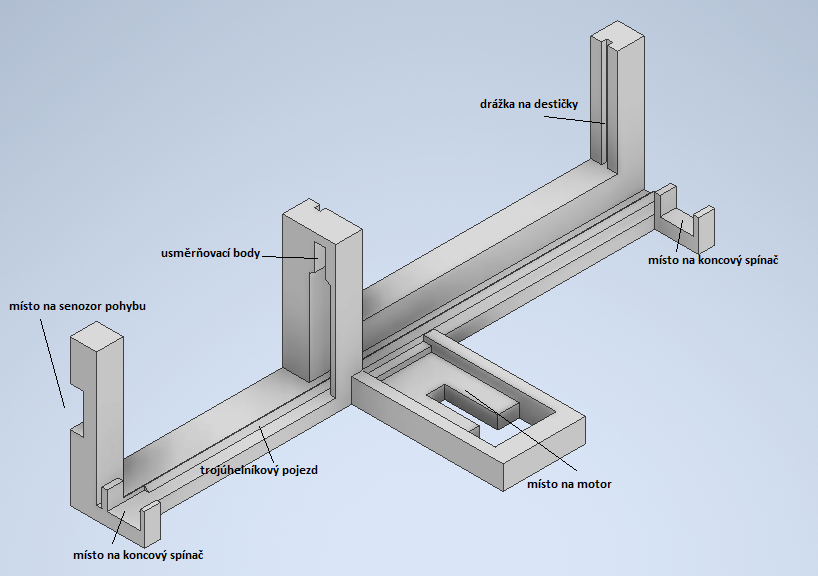
\includegraphics[width=0.7\linewidth]{image/konstrukce.png}
		\caption{Model konstrukce}
		\label{fig:konstrukceobr}
	\end{figure}
	
	\subsection{Modelování brány}
	
	\noindent V procesu modelování brány jsem vytvořil samotnou bránu, vybavil ji trojúhelníkovou drážkou pro pojezd a výstupkem pro kontakt s koncovým spínačem. \\
	
	\begin{figure}[h]
		\centering
		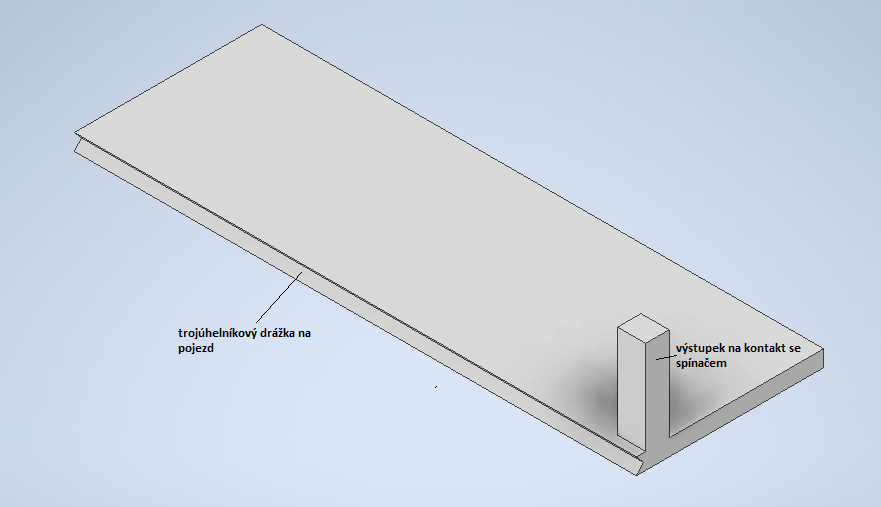
\includegraphics[width=0.7\linewidth]{image/brana.png}
		\caption{Model brány}
		\label{fig:branaobr}
	\end{figure}
	
	\newpage	
	
	\subsection{Modelování ozubeného kolečka a ozubené lišty}
	
	\noindent Pro ozubené kolečko jsem vytvořil obdélníkovou díru pro umístění motoru a kolem obvodu kola jsem vytvořil zuby. Ozubená lišta má stejnou délku jako brána a je opatřena zuby shodnými s těmi na ozubeném kolečku. \\
	
	\begin{figure}[h]
		\centering
		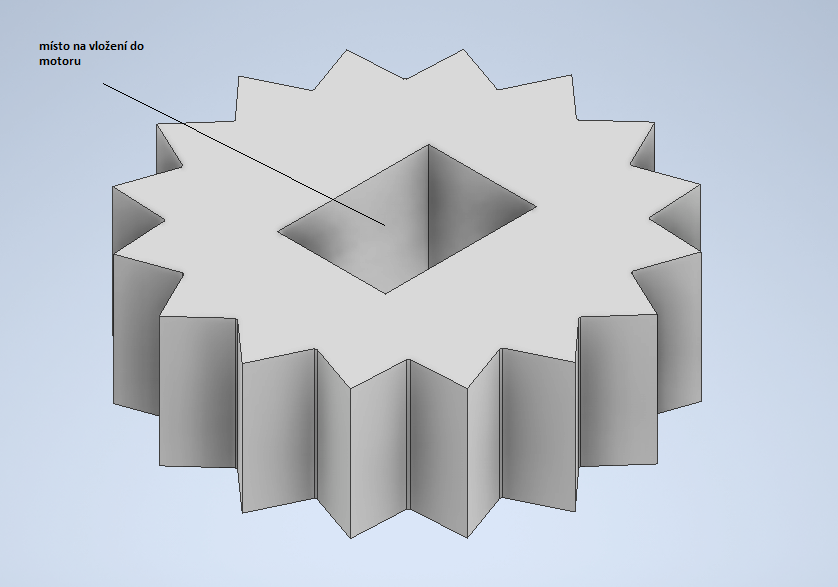
\includegraphics[width=0.7\linewidth]{image/ozubene-kolecko.png}
		\caption{Model ozubeného kolečka}
		\label{fig:ozubenekoleckoobr}
	\end{figure}
	
	\begin{figure}[h]
		\centering
		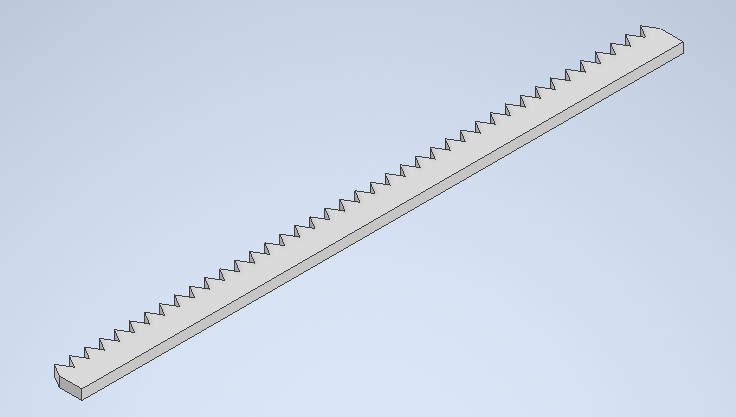
\includegraphics[width=0.7\linewidth]{image/ozubena-lista.png}
		\caption{Model ozubené lišty}
		\label{fig:ozubenalistaobr}
	\end{figure}
	
	\newpage
	
	\subsection{Modelování destiček a čepiček}
	
	\noindent Na destičky jsem přidal malé výčnělky na obou koncích, vytvářející malý rozestup mezi jednotlivými destičkami. V čepičkách je vyhrazeno místo pro LED diody a prostor pro drátky. Tyto drátky vedoucí k diodám jsou odděleny tak, aby nedošlo k dotyku mezi kladným a záporným pólem. \\
	
	\begin{figure}[h]
		\centering
		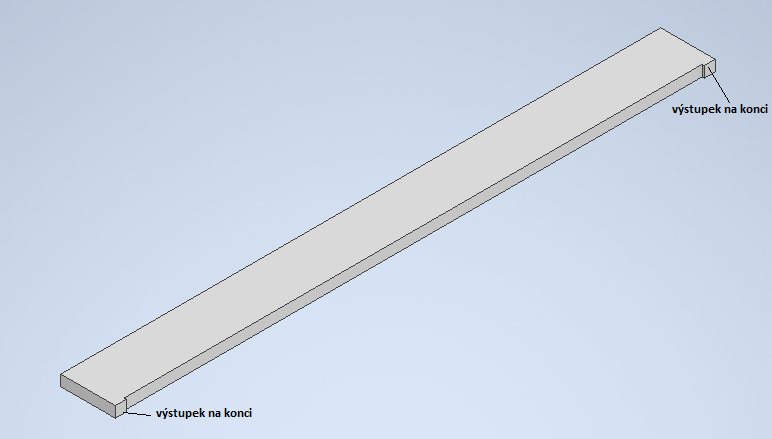
\includegraphics[width=0.7\linewidth]{image/desticka.png} 
		\caption{Model destičky}
		\label{fig:destickaobr}
	\end{figure}

	\begin{figure}[h]
		\centering
		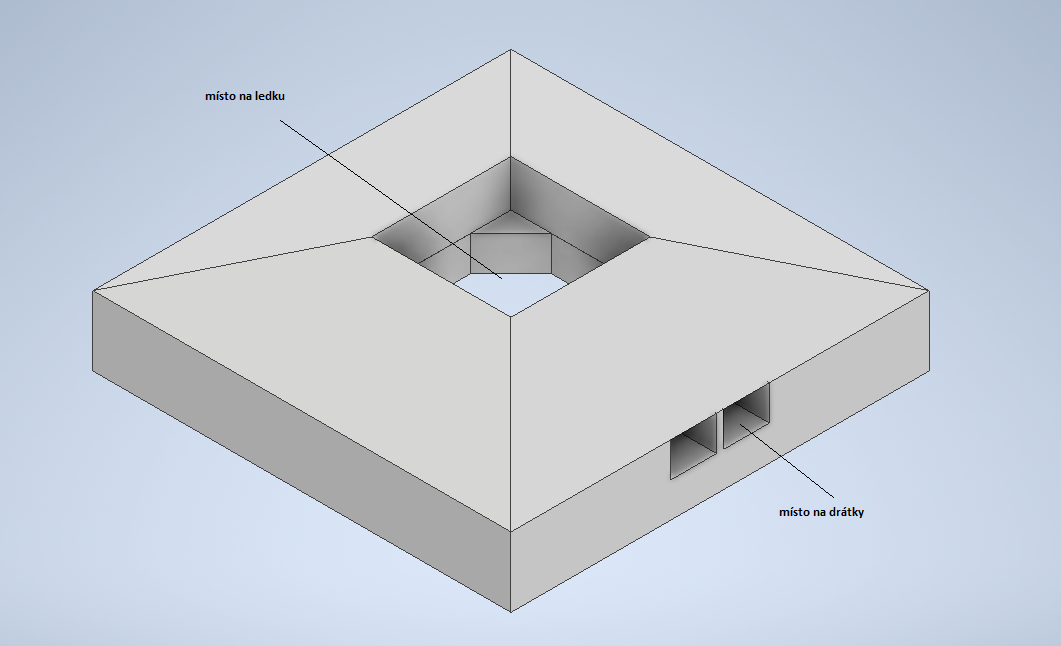
\includegraphics[width=0.7\linewidth]{image/cepicka.png}
		\caption{Model čepičky}
		\label{fig:cepickaobr} 
	\end{figure}
	
	\newpage
	
	\section{3D tisk}
	
	\noindent 3D tisk je inovativní výrobní proces, který umožňuje vytvářet třírozměrné objekty vrstvu po vrstvě na základě digitálního modelu. Tento postup eliminuje potřebu tradičního odstraňování materiálu a umožňuje vytvářet komplexní a přesné objekty s různorodými geometriemi. 3D tisk může využívat různé materiály, včetně plastů, kovů, keramiky a~biologických tkání, což poskytuje široké možnosti aplikací od průmyslové výroby a prototypování po zdravotní péči a výzkum. Tento inovativní proces zrychluje vývojové cykly a~umožňuje tvorbu unikátních a složitých designů s minimálním odpadem. \\
	
	\section{Sestavování modelu}
	
	\noindent Připevnil jsem ozubenou lištu na bránu. Motor s ozubeným kolečkem, destičky, čepičky, koncové spínače a senzor pohybu jsem přilepil na vytiskutý model pomocí tavící pistole. Nakonec jsem celý model přilepil na dřevěné desky, kde jsem rovněž přidal dvě kontaktní pole, h-můstek a následně vše zapojil. \\
	
	\begin{figure}[h]
		\centering
		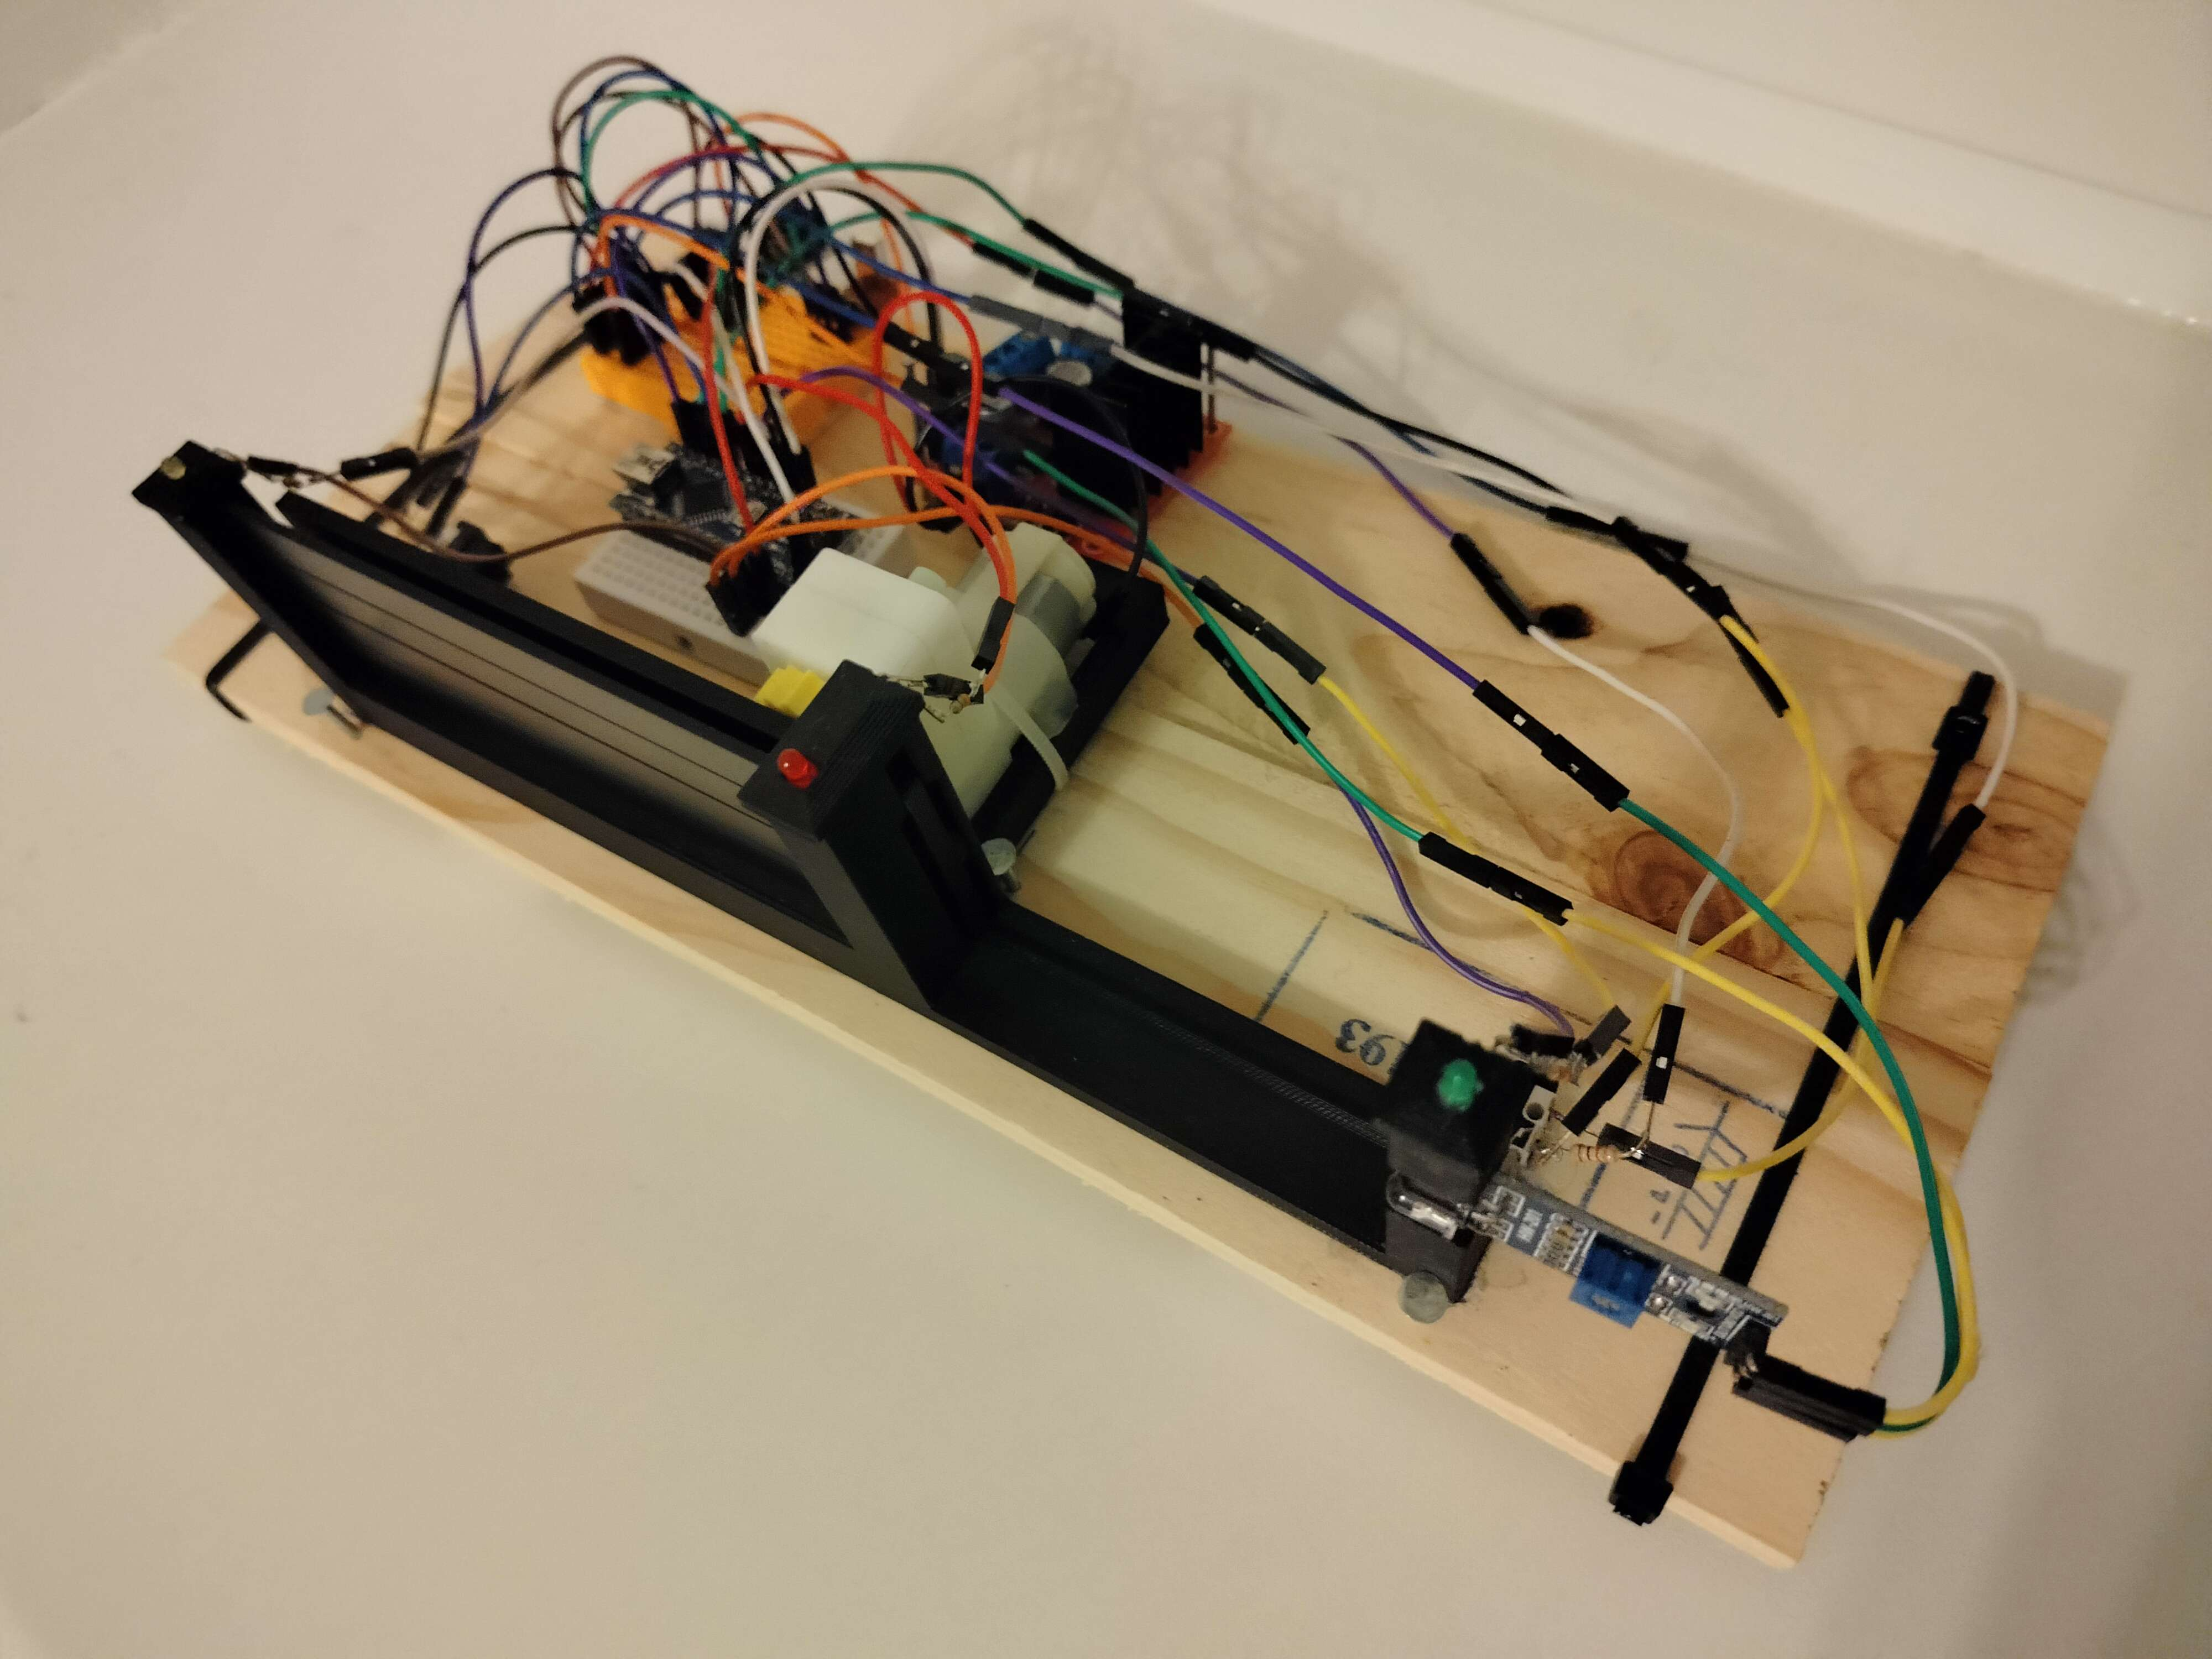
\includegraphics[width=0.7\linewidth]{image/sestava.jpg}
		\caption{Ukázka sestavení modelu}
		\label{fig:sestavaobr} 
	\end{figure}
	
	%% Stránka Hardware
	%%%%%%%%%%%%%%%%%%%%%%%%%%%%%%%%%%%%%%%
	
	\chapter{Hardware}
	\noindent Výběr hardwaru proběhl rychle a jednoduše, neboť jsem se rozhodl použít Arduino Nano, které jsme již využívali ve škole. Následně mi chyběly pouze některé komponenty, které mi vstřícně poskytl pan učitel Mgr. Marcel Godovský. \\
	
	\section{Seznam použitého hardwaru}
	
	\begin{description}
		\item  [1x Arduino Nano] Mikrokontrolér
		\item  [2x DM00 (DM 03S)] Koncové spínače
		\item  [1x L298N] H-Můstek, umožňujě měnit polarity motoru
		\item  [1x 5V motor]
		\item  [3x LED]
	    \item  [3x 330R Rezistor]
		\item  [3x 1k Rezistor]
		\item  [1x HW-201] Senzor pohybu
		\item  [1x VS1838B] IR přijímač
		\item  [1x Vytisknutá konstrukce]
		\item  [1x Vytisknutá brána]
		\item  [1x Vytiskunté ozubené kolečko]
		\item  [1x Vytisknutá ozubená tyč]
		\item  [4x Vytisknuté plotové destičky]
		\item  [3x Vytisknuté čepičky na plot]
	\end{description}
	
	\newpage
	
	\section{Schéma hardwaru}
	
	\noindent Schéma je koncipováno s cílem dosáhnout co největší přehlednosti, a proto se nemusí shodovat s reálným uspořádáním komponent v modelu. \\
	
	\begin{figure}[h]
		\centering
		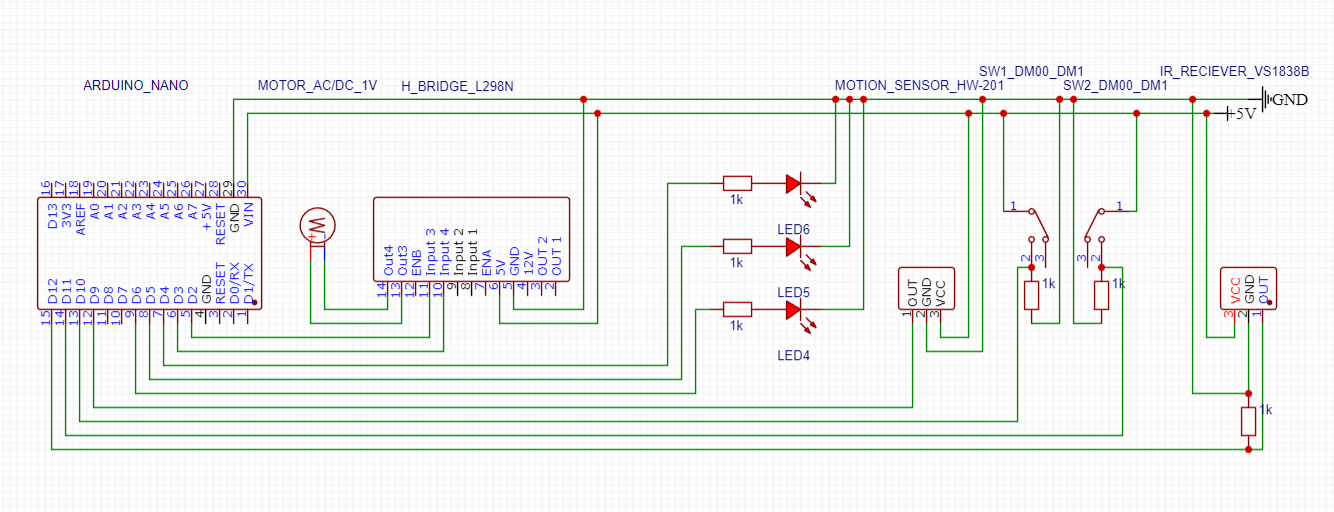
\includegraphics[width=1\linewidth]{image/schema.png}
		\caption{Schéma zapojení}
		\label{fig:schemaobr} 
	\end{figure}
	
	\section{Arduino}
	
	\noindent Arduino je open-source projekt, který je založen na snadno použitelném hardwaru a softwaru. Arduino desky mají schopnost číst různé vstupy, jako například světlo na senzoru, stisknutí tlačítka nebo dokonce zprávy z Twitteru, a přeměňovat je na odpovídající výstupy. To může zahrnovat aktivaci motoru, rozsvícení LED nebo dokonce publikaci něčeho online. S Arduino deskou můžete komunikovat pomocí instrukcí, které posíláte do mikrokontroléru. K tomu využíváte programovací jazyk Arduino a speciální vývojové prostředí Arduino Software (IDE). \\
	
	\section{Problémy s hardwarem}
	\noindent 
	Ovladač nečekaně přiděloval různé kódy na jedno tlačítko, což bylo trochu zvláštní. Toto se stávalo po určité době testování, a občas to fungovalo, zatímco jindy ne. Opravit tento problém se ukázalo být složitější, než jsem původně očekával, a tak jsem se rozhodl ho zatím neřešit. Celkově však ovladač pracuje správně přibližně 90 \% času. \\
	
	\noindent Problém s motorem a proudem vznikl, když jsem původně plánoval napájet motor přes Arduino. Nicméně jsem si neuvědomil, že Arduino poskytuje pouze omezený proud (asi 200 mA), zatímco motor, který používám, vyžaduje alespoň 500 mA. To mě vedlo k hledání externího napájení, a nakonec mi pan učitel Mgr. Marcel Godovský poskytl 5V zdroj, což je výhodné, protože z něj mohu napájet i Arduino. \\
	 
	%% Stránka Funkce Modelu Brány
	%%%%%%%%%%%%%%%%%%%%%%%%%%%%%%%%%%%%%%%

	\chapter{Funkce modelu brány}
	
	\noindent Model brány má několik základních funkcí, které by měl obsahovat každý bránový systém. To zahrnuje otevírání, zavírání a zastavování na povel z dálkového ovládání. Dále umí zastavit na základě reakce na senzor pohybu. Kromě toho model disponuje třemi LED diodami, které signalizují aktuální stav brány. \\
	
	\section{Otevření, zavření a zastavení}
	
	\noindent Pro aktivaci jedné z těchto funkcí je nezbytné stisknout příslušné tlačítko na dálkovém ovládání. Následně IR přijímač detekuje signál a přiřadí mu specifický kód. Na základě tohoto kódu tlačítka a dalších podmínek, jako jsou koncové spínače nebo senzor pohybu, rozhodne programový kód, zda se motor má roztočit či nikoli. V případě rozhodnutí pro roztočení je do motoru správně přivedeno napětí, aby se pohyboval ve správném směru. \\
	
	\noindent Aby byl IR přijímač funkční, je třeba zahrnout knihovnu \code{IRremote.h}, nastavit pin připojený k přijímači (například \code{const int RECV\_PIN = 12}), tento pin definovat pro IRrecv (\code{IRrecv irrecv(RECV\_PIN)}), vytvořit proměnnou pro ukládání výsledků a~aktivovat ho pomocí \code{irrecv.enableIRIn()}. Podmínka \code{if} uloží kód do \code{results}, pokud obdrží signál. \\
	
	\begin{lstlisting}[style=c++]	
#include <IRremote.h> //knihovna k IR prijimaci
const int RECV_PIN = 12; //definovani cisla pinu
IRrecv irrecv(RECV_PIN); //definovani pinu pro IR prijimac
decode_results results; //definovani promenne results
//povoleni IR prijimace, pise se do setupu
irrecv.enableIRIn(); 	
//podminka v loopu	
if (irrecv.decode(&results)) {
 irrecv.resume();
}		
	\end{lstlisting}

	\noindent Když máme kód tlačítka uložený, můžeme jej využít. Uložil jsem si všechny potřebné kódy do proměnných a následně je porovnával.\\
	
	\begin{lstlisting}[style=c++]
const unsigned long OPEN_CODE = 3328992116;
const unsigned long CLOSE_CODE = 404571636;
const unsigned long STOP_CODE = 204228740;
	\end{lstlisting}

	\newpage

	\noindent 
	Pro další postup je nutné konfigurovat koncové spínače; o senzoru pohybu bude podrobněji pojednáno v následující části. Nastavení pinů je identické s tím u IR přijímače, s tím rozdílem, že v setupu nastavíme tyto dva piny jako \code{INPUT}. \\
	
	\begin{lstlisting}[style=c++]
const int Button_Levy_Pin = 10;
const int Button_Pravy_Pin = 11;
		
//povoleni pinu, pise se do setupu
pinMode(Button_Levy_Pin, INPUT);
pinMode(Button_Pravy_Pin, INPUT);
	\end{lstlisting}
	
	\noindent Vytvoříme proměnné pro koncové spínače a senzor, abychom zabránili duplikaci kódu.\\
	
	\begin{lstlisting}[style=c++]
bool buttonLevyPressed = (digitalRead(Button_Levy_Pin) == HIGH);
bool buttonPravyPressed = (digitalRead(Button_Pravy_Pin) == HIGH);
bool irSensorHigh = (digitalRead(IR_Senzor_Pohybu_Pin) == HIGH);
	\end{lstlisting}

	\noindent Vytvoříme podmínky pro spouštění a zastavování motoru, kde proměnná \code{n} určuje stav motoru. První podmínka se ptá, zda je senzor aktivní či ne. Druhá podmínka kontroluje, zda je aktivní \code{STOP\_CODE}. Třetí podmínka zkoumá, zda není aktivní ani \code{OPEN\_CODE}, ani \code{CLOSE\_CODE}. S každým průchodem smyčkou se kód resetuje, a tím pádem tato podmínka začne platit, což umožní koncovým spínačům zastavit motor při jejich aktivaci. Čtvrtá podmínka se ptá, zda je vždy jeden spínač sepnutý a druhý nikoli. Toto zajistí zastavení motoru, když se jeden ze spínačů sepne. Pátá podmínka ověřuje, zda je aspoň jeden nebo žádný spínač sepnutý. Toto je implementováno z důvodu, že brána je obvykle na konci a má spínač sepnutý, nebo je uprostřed cesty a spínače nejsou sepnuté. \\
	
\begin{lstlisting}[style=c++]
if (irSensorHigh) { 
 if (results.value != STOP_CODE) { 
  if (results.value != OPEN_CODE && results.value != CLOSE_CODE) {
    if ((buttonPravyPressed && !buttonLevyPressed) || 
        (!buttonPravyPressed && buttonLevyPressed)) {
     n = 2;                         
  }
 } else if (!buttonLevyPressed || !buttonPravyPressed) { 
  n = 1;
 }
} else {
	n = 2;
 }
} else {
 n = 2;
 results.value = STOP_CODE;
}
\end{lstlisting}
	
	\newpage
	
	\noindent Točení motoru ve správném směru vyřešíme porovnáním, které tlačítko na ovladači bylo stisknuto, a přiřadíme odpovídající směr do proměnné \code{direction}. Při tomto procesu také resetujeme proměnnou \code{results}, abychom zajistili správnou funkčnost programového kódu, jak je zmíněno v posledním odstavci. \\
	

	
\begin{lstlisting}[style=c++]
if (results.value == OPEN_CODE) {
 direction = LEFT;
 results.value = 0;
} else if (results.value == CLOSE_CODE) {
 direction = RIGHT;
 results.value = 0;
}
\end{lstlisting}

	\noindent Ještě musíme definovat proměnnou \code{direction}. \\
	
\begin{lstlisting}[style=c++]
enum Direction { LEFT = 1, RIGHT = 2 };
int direction;
\end{lstlisting}	
	
	\section{Senzor na pohyb}
	
	\noindent U senzoru pohybu musíme definovat pin, ke kterému je připojen, a v setupu povolit tento pin jako \code{INPUT}. \\
	
\begin{lstlisting}[style=c++]
const int IR_Senzor_Pohybu_Pin = 9;
//povoleni pinu, pise se do setupu
pinMode(IR_Senzor_Pohybu_Pin, INPUT);
\end{lstlisting}

	\noindent Kontrolujeme stav senzoru a sledujeme, zda je ve stavu \code{HIGH} nebo \code{LOW}. Vzhledem k~tomu, že stav \code{LOW} signalizuje aktivitu, když je senzor v tomto stavu, motor se nespustí a~ nastavíme kód tlačítka na \code{STOP\_CODE}. Tímto způsobem zajistíme, že se motor okamžitě zastaví a nebude znovu spouštěn. Tato opatření jsou implementována tak, aby se předešlo situaci, kdy by brána reagovala na krátkodobou aktivaci senzoru, například při průchodu dítěte, a brána by se zastavila a ihned znovu spustila. Tímto způsobem je zajištěno, že brána zůstane zastavená po detekci aktivity. \\

\begin{lstlisting}[style=c++]
if (irSensorHigh) {
 /* chybejici kod */
} else {
 n = 2;
 results.value = STOP_CODE;
}
\end{lstlisting}
	
	\newpage
	
	\section{LED indikátory a motor}
		
	\noindent Zapnutí motoru a LED na základě proměnných \code{n} a \code{direction} začíná tím, že znovu definujeme a nastavujeme piny. Tyto piny jsou poté povoleny v setupu, přičemž všechny jsou nastaveny jako \code{OUTPUT}. \\
	
\begin{lstlisting}[style=c++]
const int LED_Uprostred_Pin = 6;
const int LED_Vlevo_Pin = 4;
const int LED_Vpravo_Pin = 5;
const int Motor_Pravy_Pin = 2;
const int Motor_Levy_Pin = 3;

//povoleni pinu, piseme do setupu
pinMode(LED_Uprostred_Pin, OUTPUT);
pinMode(LED_Vlevo_Pin, OUTPUT);
pinMode(LED_Vpravo_Pin, OUTPUT);
pinMode(Motor_Pravy_Pin, OUTPUT);
pinMode(Motor_Levy_Pin, OUTPUT);
\end{lstlisting}
	
	 \noindent  Pro aktivaci motoru potřebujeme nastavit jeden pin na \code{HIGH} a druhý na \code{LOW}. Tuto konfiguraci řídí proměnná \code{n}, která určuje, zda se motor má točit, a proměnná \code{direction}, která určuje směr otáčení. Pro aktivaci LED diod postupujeme obdobně. Nakonec přidáváme \code{delay(180)} pro správnou funkčnost koncových spínačů, které reagují příliš rychle. Toto zpoždění bylo zavedeno k úpravě problémů s přílišnou citlivostí spínačů, které vedly k nežádoucím krátkým pohybům brány. \\

	
\begin{lstlisting}[style=c++]
 digitalWrite(LED_Uprostred_Pin, n == 1);
 digitalWrite(LED_Vlevo_Pin, n == 1 && direction == LEFT);
 digitalWrite(LED_Vpravo_Pin, n == 1 && direction == RIGHT);
 digitalWrite(Motor_Pravy_Pin, n == 1 && direction == LEFT);
 digitalWrite(Motor_Levy_Pin, n == 1 && direction == RIGHT);
	
 if (n == 1) {
  delay(180);
 }
\end{lstlisting}

	\newpage

	\section{Optimalizace kódu}
	
	\noindent Pro optimalizaci kódu začneme definováním proměnných úplně nahoře (kromě knihoven). Následně pokračujeme funkcí \code{setup()}, kde povolujeme piny a definujeme akce. Dále máme vlastní funkci \code{handleLEDsAndMotors()}, která se stará o zapínání pinů pro LED diody a motor. Následuje funkce \code{checkIRSensorAndButtons()}, kde se nachází rozsáhlá sada podmínek. Dále je tu funkce \code{processIRResults()}, ve které určujeme směr. Na závěr máme funkci \code{loop()}, kde jsou volány všechny vlastní funkce, a kód ovladače je uložen do proměnné \code{results}. \\
	
	
\begin{lstlisting}[style=c++]
void loop() {
 if (irrecv.decode(&results)) {
  irrecv.resume();
 }
 checkIRSensorAndButtons();
 processIRResults();
 handleLEDsAndMotors();
}
\end{lstlisting}
	
	\section{Ovládání brány}
	\noindent Pomocí ovladače odesíláme signál, který programový kód vyhodnotí a přiřadí kód tlačítka do proměnné \code{results} (\code{OPEN\_CODE, STOP\_CODE, CLOSE\_CODE}). Pokud je kód tlačítka roven \code{OPEN\_CODE} a splňují se všechny podmínky, motor se zapne a brána se otevře. V případě, že kód tlačítka odpovídá \code{CLOSE\_CODE} a všechny podmínky jsou splněny, motor se zapne a brána se zavře. Při shodě s kódem \code{STOP\_CODE} se nic nestane, motor zůstane vypnutý. Pokud je motor aktivní a senzor pohybu se aktivuje, motor se zastaví a~už se nespustí. \\
	
	%% Stránka Závěr
	%%%%%%%%%%%%%%%%%%%%%%%%%%%%%%%%%%%%%%%
	
	\newpage
	
	\chapter*{Závěr}
	\addcontentsline{toc}{chapter}{Závěr}
	
	\noindent Cílem projektu bylo vytvořit model posuvné brány s elektrickým pohonem, kterou lze ovládat pomocí dálkového ovládání. Model byl vymodelován v programu Autodesk Inventor, následně vytisknut na 3D tiskárně a spolu s hardwarem sestaven. Pro realizaci byl využit mikrokontroléř Arduino Nano, který byl naprogramován. \\
	
	\noindent Podle mého názoru jsem cílů projektu dosáhl. Během procesu práce jsem získal dovednosti efektivního modelování v programu Autodesk Inventor a naučil se vhodně vytvářet modely pro snadné 3D tisknutí. Dále jsem zdokonalil své programátorské dovednosti a~získal zkušenosti s Arduinem. Pro budoucí vylepšení plánuji přidat kameru, která bude snímat SPZ a na základě těchto údajů otevírat bránu. Také mám v úmyslu vytvořit mobilní aplikaci, která bude fungovat jako dálkový ovladač. \\
		
		
		\renewcommand{\bibname}{Seznam použitých zdrojů}
		%% literatura
		\begin{thebibliography}{99}
			\bibitem{citacePRO}\textit{Citace PRO} [online]. Citace.com, 2020 [cit. 2020-08-31]. Dostupné z: \url{https://www.citacepro.com}
			\bibitem{Arduino}\textit{Arduino} [online]. Arduino.cc, 2024 [cit. 2024-1-8]. Dostupné z: \url{https://www.arduino.cc}
			\bibitem{easyEda}\textit{EasyEDA} [online]. easyeda.com, 2024 [cit. 2024-1-8]. Dostupné z: \url{https://easyeda.com/}
			\bibitem{inventor}\textit{Autodesk Inventor} [online]. autodesk.cz/products/inventor/, 2024 [cit. 2024-1-8]. Dostupné z: \url{https://www.autodesk.cz/products/inventor/}
			\bibitem{canva}\textit{Canva} [online]. canva.com, 2024 [cit. 2024-1-9]. Dostupné z: \url{https://www.canva.com}
		\end{thebibliography}
		
		%% obrázky 
		\listoffigures
		
		\appendix %% začínají přílohy
		
		\titleformat{\chapter}[block]{\scshape\bfseries\LARGE}{Příloha \thechapter}{10pt}{\vspace{0pt}}[\vspace{-22pt}] %% nastavení nadpisu u příloh
		
		
		
	\end{document}